\section{Passing parameters to linux kernel module}

\text{Using \textit{module\_param} function to declare parameters}

\textbf{Example code below}
\begin{lstlisting}[style=CStyle]
    #include <linux/kernel.h>
    #include <linux/module.h>
    
    MODULE_LICENSE("GPL");
    
    char *name = "Danny";
    int count = 0;
    module_param(name, charp, S_IRUGO);
    module_param(count, int, S_IRUGO);
    
    
    static int test_arguments_init(void) {
        printk(KERN_INFO"%s: In init\n", __func__);
        printk(KERN_INFO"%s: name: %s\n", __func__, name);
        printk(KERN_INFO"%s: pass count: %d\n", __func__, count);
    
        return 0;
    }
    
    
    static void test_exit(void) {
        printk(KERN_INFO"%s: In exit: \n", __func__);
    }
    
    
    
    module_init(test_arguments_init);
    module_exit(test_exit);
    
    MODULE_AUTHOR("Danny Deng");
    MODULE_DESCRIPTION("Argument parsing example");    
\end{lstlisting}

\text{}

\textbf{Each parameters can declare different permission}
\begin{center}
    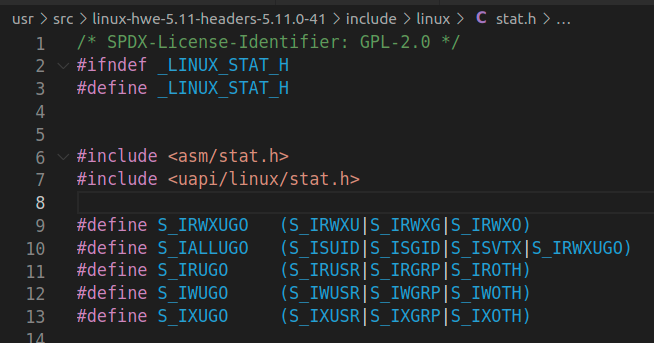
\includegraphics[width=\linewidth]{images/kernel_permission.png}
\end{center}

\textbf{The macro value define below}
\begin{lstlisting}[style=CStyle]
#define S_IRWXU 00700
#define S_IRUSR 00400
#define S_IWUSR 00200
#define S_IXUSR 00100

#define S_IRWXG 00070
#define S_IRGRP 00040
#define S_IWGRP 00020
#define S_IXGRP 00010

#define S_IRWXO 00007
#define S_IROTH 00004
#define S_IWOTH 00002
#define S_IXOTH 00001
\end{lstlisting}

\text{S\_I + R/W/X + USR/GRP/OTH}
\begin{itemize}
    \item R: Read
    \item W: Write
    \item X: Execute
    \item USR: User
    \item GRP: Group
    \item OTH: Other
\end{itemize}

\textbf{Insert the kernel module, and feed the parameter}
\begin{lstlisting}[style=bashStyle]
    $ sudo insmod passing_simple_count.ko count=10 name=Danny
\end{lstlisting}

\textbf{Remove the kernel module}
\begin{lstlisting}[style=bashStyle]
    $ sudo rmsmod passing_simple_count
\end{lstlisting}

\textbf{Show the result}
\begin{lstlisting}[style=bashStyle]
    $ dmesg
\end{lstlisting}

\begin{center}
    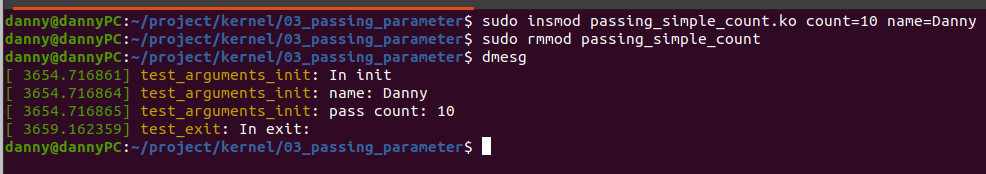
\includegraphics[width=\linewidth]{images/03_pass_para_terminal.png}
\end{center}



